\chapter{Criptosistemas clásicos}

La criptografía tiene como objetivo resolver el siguiente problema:

\begin{figure}[h]
	\begin{center}
		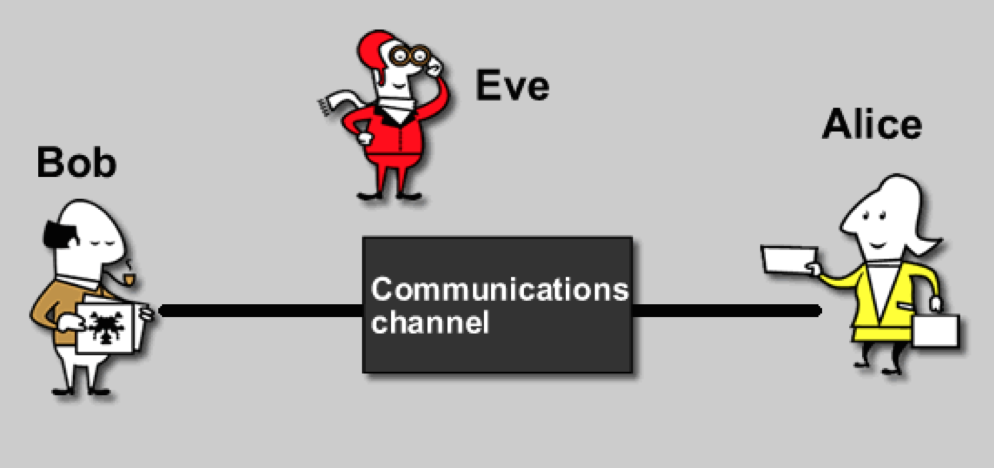
\includegraphics[width=0.5\textwidth]{img/aliceBobEve.png}
		\caption{Cómo enviar un mensaje de manera segura entre Bob y Alice por un canal al que Eve tiene acceso}
	\end{center}
\end{figure}


El objetivo es garantizar tanto la confidencialidad del mensaje (Eve no es capaz de saber qué se están diciendo) como de autentifiación (Alice está segura de que es Bob quien mandó el mensaje y viceversa)

A lo largo de este capítulo veremos los métodos que han sido empleados a lo largo de la historia para lograr este objetivo.

	\section{Esteganografía}

		Intentar ocultar la existencia del mensaje. Es un método con origen muy antigüo (~486-425 a.C)

	\section{Criptografía}
		\begin{defn}[Criptografía]
		Tradicionalmente se ha definido como el ámbito de la criptología el que se ocupa de las técnicas de cifrado o codificado destinadas a alterar las representaciones lingüísticas de ciertos mensajes con el fin de hacerlos ininteligibles a receptores no autorizados.

		El primer método de criptografía data del siglo V antes de cristo
		\end{defn}

		La mayoría de estos métodos se basaban en transposición.

		\begin{defn}[Transposición]
			Cambio en el orden de las letras de un mensaje
		\end{defn}

		\subsection{El criptosistema de Cesar}

			Se utiliza la sustitución como método de encriptación, normalmente cambiando cada letra por su correspondiente al desplazarse $d$ espacios atrás en el abecedario. Por ejemplo:
			\begin{center}
			\begin{tabular}[h]{c|c}
			sin cifrar & cifrado \\ \hline
			A & D\\
			B & E\\
			C & F\\
			... & ...
			\end{tabular}
			\end{center}

		\subsection{Formalización}

		Vamos a ver cómo denominamos formalmente los elementos que intervienen en un proceso de cifrado:
		\begin{itemize}
			\item \textbf{Mensajes}

			Tenemos dos diferentes mensajes en todo proceso de cifrado
			\begin{enumerate}
			\item M = Mensajes en claro
			\item C = Mensajes cifrados
		\end{enumerate}

		\item \textbf{Alfabeto}
		Tendremos un alfabeto o dos, dependiendo de si los alfabetos de M y C son el mismo o no.

		Ejemplos de alfabetos serían:
		\begin{itemize}
			\item $A = \{A,B...Z\}$
			\item $A = \{0,1\}$
			\item $A = \{A,B...Z,\hdots,\text{?`},\text{?},1,2,3,\hdots,9,0\}$
			\item $A = $ Código ASCII
		\end{itemize}

		\item \textbf{Funciones para cifrar}

		Serán funciones de la forma $f: M \rightarrow C$ donde $f$ es inyectiva

		\item \textbf{Funciones para descifrar}

		Serán funciones de la forma $f^{-1}: C \rightarrow M$ donde $f$ es la misma función empleada para cifrar el mensaje.
		\end{itemize}

		Para que pueda llevarse a cabo la comunicación entre $A$ y $B$, A debe conocer $f$ y $B$ debe conocer $f^{-1}$. A envía un mensaje $m\in M$ a $B$ usando $f(m)=c$ y enviando $c$. $B$ puede obtener el mensaje calculando $f^{-1}(c) = m$.

		En este modelo, romper el sistema de cifrado equivale a que un tercero averigüe $f^{-1}$.


		\textbf{¿Podemos usar más de una función para cifrar?}

		En el sistema de Cesar se puede cambiar, por ejemplo, la longitud desplazmiento por el abecedario al realizar la encriptación, aunque no hay muchas posibilidades.

		\begin{defn}[Criptosistema]
			Colección de functiones para cifrar. Se trata de funciones de la forma
			\[\appl{f_e}{M_e}{C_e}\]
		\end{defn}


		\begin{example}{\textbf{Como romper la criptografía Cesar}}

			Se puede romper "facilmente" la criptografía Cesar con análisis de frecuencias. Por ejemplo, en castellano la letra más frecuente es la E, con un 13,68\%, sabiendo la letra más frecuente de un mensaje cifrado se puede calcular la distancia entre esa y la E y muy probablemente hayamos hallado la clave de cifrado.

			La fiabilidad de este método puede verse mermada por la genericidad del texto cifrado. Si es corto y si habla de un tema en particular es posible que las frecuencias varíen respecto a otros textos genéricos en Español.

			De hecho, por ejemplo, en el manual de UNIX la frecuencia de la letra e baja al 9\% dejando a la letra relegada al cuarto puesto, por detrás de la t, la n y la i.

		\end{example}


		Veamos la frecuencia general de distintos grupos de letras en ingles.

		\begin{tabular}[h]{r|c|c}
			\textbf{grupos} & \textbf{frec} & \textbf{rango} \\ \hline
			e & 12.7\% & 12.7 \\
			taoiushr & 56.9 & 6-9 \\
			cumwfgypb & 19.9 & 1.5 - 3 \\
			vkjxqz & 2.2 & < 1
		\end{tabular}

		\section{Criptosistema afín (sobre letras)}

			\begin{defn}[Cifrado afín]
			El cifrado afín también se le llama cifrado de transformación afín o cifrado monoalfabético genérico. Es un tipo de cifrado por sustitución en el que cada símbolo del alfabeto en claro (el alfabeto del texto en claro) es sustituido por un símbolo del alfabeto cifrado (el alfabeto del texto cifrado) siendo el número de símbolos del alfabeto en claro igual que el número de símbolos del alfabeto cifrado. Para hallar el símbolo del alfabeto cifrado que sustituye a un determinado símbolo del alfabeto en claro, se usa una función matemática afín en aritmética modular. Para poder aplicar la función matemática lo primero que hay que hacer es asignar un orden que a cada símbolo de cada uno de los alfabeto le asocie un número de orden.
			\end{defn}

			Si tenemos un alfabeto de N letras $\leftrightarrow \mathbb{Z}/N$ y denominamos a las claves: $a,b \in \mathbb{Z}/N$, tenemos que el proceso de cifrado puede representarse mediante la siguiente fórmula matemática:

			\begin{align*}
				f_{a,b} :&  \mathbb{Z}/N\to \mathbb{Z}/N\\
				& x \rightarrow ax + b
			\end{align*}

			\subsection{¿Para qué valores de a,b es $f_{a,b}$ inyectiva?}

			Para verlo calculamos $f^{-1}_{a,b}$

			$$ax+b = y$$
			$$ax = y - b$$

			Si $a \in U(\mathbb{Z}/N)
			\implies
			x = a^{-1} (y-b) \implies
			x = a^{-1}y - a^{-1}b$


			$$f^{-1}_{a,b} = f_{a^{-1},-a^{-1}b}$$

			Así hemos demostrado que:

			\begin{enumerate}
				\item $a \in U(\mathbb{Z}/N) \Rightarrow f_{a,b}$ inyectiva
				\item En ese caso si $e = (a,b)$ es la clave para cifrar $\Rightarrow d = (a^{-1},-a^{-1}b)$ es la clave para descifrar.
			\end{enumerate}

			Usando la definición de inyectiva:

				$$ \exists \alpha \in q : a \alpha = 1 \Leftrightarrow a \alpha + b = 1 + b $$

			Así llegamos a la conclusión de que en realidad el par $(a,b)$ tiene ciertas restricciones:

			$$ E = \{ (a,b): a \in U(\mathbb{Z}/N), b \in \mathbb{Z}/N \} $$

			$$ \#E = \#U(\mathbb{Z}/N) * \#\mathbb{Z}/N $$


			\begin{prop}
				Sea $a \in \mathbb{Z}/N : a \in U(\mathbb{Z}/N) \Leftrightarrow (a,N) = 1$ (son primos entre si).

				\begin{proof}

					\textbf{$\Rightarrow$}

					$$\exists \alpha \in \mathbb{Z}/N : a \alpha \equiv 1 \mod n \Rightarrow \exists k : a\alpha + kN = 1$$

					$$\text{Si } (a,N) \neq 1 \Rightarrow \exists p \text{ primo } : p | a, N \Rightarrow p | ax + kN \Rightarrow p | 1 \text{ lo cual es imposible.} $$

					\textbf{$\Leftarrow$}

					$(a,n) = 1$. Esto se demuestra usando el algoritmo de euclides.

				\end{proof}
			\end{prop}


			Volvemos entonces al número de claves ya que sabemos como calcularlo:

			$$ \#E = \#U(\mathbb{Z}/N) * \#\mathbb{Z}/N = \phi(N)*N $$


			\subsection{La función de Euler}

				\begin{defn}[Función de Euler]
				La función φ de Euler (también llamada función indicatriz de Euler) es una función importante en teoría de números. Si n es un número entero positivo, entonces φ(n) se define como el número de enteros positivos menores o iguales a n y coprimos con n, es decir, formalmente se puede definir como:

				\[φ(m) = \left| \{n \in \nat \tq n \leq m \wedge mcd(m,n)=1\}\right|\]

				En el caso de que queramos calcular la función de Euler de un número primo $p$ tenemos:

				$\phi(p) = p-1$

				$\phi(p^n) = p^{n} - p^{n-1} = p^{n-1} (p-1) = p^{n}(1- \frac{1}{p})$

				Como es una función multiplicativa:

				$\phi(N) =N \Pi \phi(P_i^{n_i}) = \Pi P_i^{n_i} n_i \Pi \left(1- \frac{1}{p_i}\right) = N \Pi\left(1 - \frac{1}{p_i}\right)$
				\label{func:Euler}
				\end{defn}

\begin{figure}[h]
	\begin{center}
		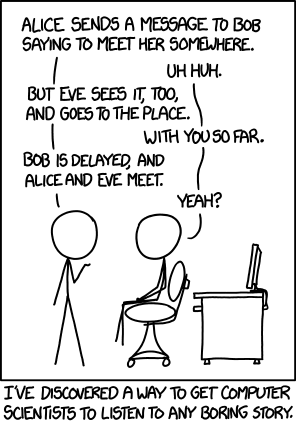
\includegraphics[width=0.5\textwidth]{img/protocol.png}
	\end{center}
\end{figure}

Veamos un ejemplo de como un espía podría realizar un ataque contra un usuario que emplea este sistema de cifrado.
\begin{example}
El objetivo es conseguir conocer los valores $a$ y $b$ que han sido empleados para lo que deberemos resolver un sistema de dos ecuaciones de dos incógnitas, una vez hemos obtenido una muestra de un texto cifrado y su original sin cifrar.

Como, en teoría, el atacante no tendría acceso al texto original, empleará una tabla de frecuencias que, en un texto en inglés, nos dice que las letras más frecuentes son la E y la T.

Ahora podemos estudiar el texto cifrado y ver que las letras más usadas son, respectivamente, U y D. Por tanto, convirtiendo estas letras en sus correspondientes números (según la posición que ocupan en el alfabeto inglés) tenemos el siguiente sistema de ecuaciones:
\[
\left\{
20α + β = 4\atop
3α +β = 19
\right.\]

Que, si restamos a la primera ecuación la segunda y nos apoyamos en el hecho de que estamos trabajando en $\ent_{26}$ nos queda:
\[
\left\{
20α + β = 4\atop
17α = 11
\right.\]

Ahora debemos encontrar el inverso multiplicativo de 17 trabajando en módulo 26, para lo que emplearemos el algoritmo de Euclides.

\begin{enumerate}
\item $26 = 17 + 9$
\item $17 = 9 + 8$
\item $9 = 8 + 1 $
\item $8 = 8 \cdot 1 + 0$
\end{enumerate}

Como al final hemos obtenido un $+0$ el propio algoritmo de Euclides nos garantiza que existe el inverso multiplicativo modulo 27 de 17.

Ahora aplicamos el algoritmo de Euclides para obtener el inverso y para ello expresamos cada resto sustituyendo en la fórmula resultando el resto siguiente. Es decir:
\[1 = 9 - 8 = 9- (17-9) = 2 \cdot 9 - 17 = 2 \cdot (26 - 17) - 17 = 2 \cdot 26 - 3 \cdot 17 = -24 \cdot 26 + 23 \cdot 17 \implies \]
\[\implies 1 + 24 \cdot 26 = 23 \cdot 17 \implies 1 = 23 \cdot 17\]
Con ello llegamos a que:
\[\frac{1}{17} = 23 \implies α = 23 \cdot 11 = 19 \& β = 14\]
\end{example}

Veamos otro ejemplo un poco más interesante.
\begin{example}
En este caso consideramos que el conjunto de símbolos válidos empleados por el emisor al escribir el texto original son: el alfabeto inglés, el espacio y el símbolo de interrogación.

En este caso el espía intercepta un mensaje y encuentra que los símbolos más habituales en ese mensaje han sido la B y ?. En este caso no podemos emplear la misma tabla de frecuencias que en el ejemplo anterior, puesto que el alfabeto inicial ha cambiado.

Con las nuevas condiciones tenemos que las letras más habituales se relacionan de la forma:
\[B \to \_ \]
\[? \to E\]
que nos lleva al sistema de ecuaciones:
\[
\left\{
α+β = -2\atop
-α+β = 4
\right. \implies 2α = -6\]

Pero en esta ocasión no podemos emplear el algoritmo de Euclides, pues el 2 no es coprimo con 6 ni con su inverso aditivo.

En esta ocasión, el problema se debe a que estamos trabajando en $\ent_{28}$ que es un cuerpo con divisores de 0 y, por tanto, el sistema de ecuaciones no tendrá una única solución sino varias. En este caso nos quedan que son soluciones posibles los pares de valores:
\[α=11, \ β=15 \;\;\; \& α=25 \ β=1\]

Ahora lo que podríamos hacer es probar ambas combinaciones y ver cuál de ellas nos permite obtener un texto original con sentido.

Otra posibilidad es acudir a la tabla de frecuencias y ver cuál de los dos sistemas nos permite obtener la siguiente letra más frecuente. Si las cosas funcionan bien, sólo uno de los dos sitemas nos funcionará.

Así, tomamos la I, que es la tercera letra más habitual en el mensaje cifrado y vemos que nuestros valores de α y β nos llevan a que la letra original podría ser T o F.

Puesto que la T es una de las letras menos habituales, la hipótesis razonable es pensar que los valores correctos de α y β es $(11,15)$.
\end{example}

Tras estos ejemplos hay una duda que debería surgir directamente en el lector. En ambos ejemplos nos hemos basado en un absoluto conocimiento acerca del sisteme alfanumérico empleado en el mensaje original, pero esto no es realista.

Para explicar esto debemos fijarnos en el \textbf{Principio de Kerkhoffs} que dice:
\begin{prop}[Principio de Kerkhoffs]
No puede requerirse que un criptosistema sea secreto. Tiene que poder caer en manos del enemigo sin que esto suponga un inconveniente.

Es decir: la seguridad del sistema tiene que depender UNICAMENTE de mantener secretas las claves.
\end{prop}

Recordemos que el sistema de Cesar tenía el gran inconveniente de que había muy pocas posibilidades. Es decir, con hacer 26 pruebas se puede obtener el mensaje original a partir de un mensaje cifrado.

Este problema se ha relajado mediante el empleo de la criptografía afín pero, como acabamos de ver, sigue siendo sencillo descifrar un mensaje.

Con el fin de mejorar la seguridad aparece el \textbf{Criptosistema de sustitución}

\section{Criptosistema de sustitución}

Este sistema simplemente consiste en una mejora del sistema César. En lugar de desplazar todas las letras del alfabeto lo que se hace es tomar una reordenación del mismo.

El principal problema del sistema de crifrado César es que sólo existen 26 posibles claves (correctamente hay N posibles claves siendo N el tamaño del alfabeto empleado), que es un número muy pequeño.

Con el sistema de sustitución simple pasamos a tener un total de $26! = 4 \cdot 10^{26}$ posibles claves. Para que nos hagamos una idea de lo desorbitadamente grande que es este número, tened en cuenta que la NASA calculó que con un procesador de Intel de los más potentes hasta la fecha de 2009, serían necesarios más de 10.000 años para probar todas las posibles claves.

Aún así, el sistema de cifrado por sustitución sigue siendo vulnerable a ataques por análisis de frecuencias.

\section{Definción de Criptabeto}

El problema de los sistemas que hemos visto, y sobre todo del último, es que es necesario que el emisor y el receptor del mensaje se pongan de acuerdo en la relación alfabeto original - alfabeto crifrado que se va a emplear.

Para llevarlo a cabo existen diferentes alternativas:
\begin{itemize}
\item \textbf{Frase clave}

\item \textbf{Palabra clave - lectura clave}
\end{itemize}

En este punto es interesante mirar las transparencias de la asignatura que pueden encontrarse en moodle.

\section{Lucha contra el análisis de frecuencias}
Una posible forma de hacer el sistema menos vulnerable a este tipo de ataques consiste en cifrar las letras por grupos. Por ejemplo, podemos agruparlas de 2 en 2.

Una vez decidimos cómo de grande es el grupo de letras que vamos a juntar (y por ahora suponemos es 2) podemos cifrarlo de dos formas diferentes:

\begin{itemize}
\item \textbf{Pares de letras vistas como números de dos cifras en base 26}

En este caso emplearíamos funciones del tipo
\[f(m)= (Am + B) \ mod \ 26^2, \;\; A,B \in \ent_{26^2}\]

\item \textbf{Pares de letras vistas como vectores de dimensión 2 sobre $\ent_{26}$}

Este sistema nos permite emplear matrices y se conoce como \textbf{Criptosistema de Hill}

\[ f(m_1\ m_2) = \left( \begin{array}{cc}
a & b \\
c & d  \end{array} \right) \cdot\left( \begin{array}{c}
m_1 \\
m_2  \end{array} \right) \ \text{ con } a,b,c,d \in \ent_{26}\]
\end{itemize}

Ambos sistemas pueden extenderse a alfabetos más grandes y a agrupaciones de letras mayores. Sin embargo, el criptosistema de Hill (también conocido como lineal) requiere que la matriz sea invertible, pues de lo contrario el mensaje no sería descifrable.

Veamos cuándo la matriz será invertible, teniendo en cuenta qué significa ser invertible en el cuerpo en que estamos trabajando.

\begin{prop}
Una matriz con coeficientes en $\ent_{N}$ tiene inversa si y sólo si el determinante de la matriz pertenece al conjunto de las unidades de $\ent_{N}$
\end{prop}
\begin{proof}
Vamos a demostrar los dos sentidos de la implicación:
\begin{itemize}
\item $\Rightarrow$
Suponemos que existe la matriz inversa de $A$, $A^{-1}$. Entonces sabemos que
\[det(A\cdot A^{-1})=det(A)\cdot det(A^{-1}) = det(I) = 1 \implies det(A) \in U(\ent_{N})\]
\item $\Leftarrow$
Antes de poder ver esta demostración debemos recordar, de lo que aprendimos en primero, que si multiplicmaos la matriz $A$ por la traspuesta del adjunto obtenemos una matriz diagonal con todos los elementos no nulos iguales a $det(A)$

Una vez tenemos esto es claro ver que
\[A \left( \frac{1}{det(A)}Adj(A)^t \right) = I\]

Es decir, una vez sabemos que el determinante de la matriz pertenece al conjunto de unidades de $\ent_N$ sabemos que tiene inverso, lo que nos permite escribir $\frac{1}{det(A)}$ que es necesario para la definición constructiva que todos conocemos de matriz inversa.
\end{itemize}
\end{proof}

La cuestión que surge ahora es bastante obvia. ¿Y si al exigir que la matriz sea invertible estamos acotando demasiado el espacio de claves posibles?. Vamos a contar cuántas matrices hay invertibles para cada $n$ dado.

De aquí en adelante $N$ será el número de letras que estamos agrupando, es decir, el orden de la matriz y $n$ será el tamaño del alfabeto empleado, que denotaremos como $p$ siempre que sea primo.
\begin{itemize}
\item \textbf{Agrupamos las letras por parejas}

En este caso tendremos que el determinante sería de la forma $ad-bc$.

Ahora vamos a contar cuántas matrices hay que tengan determinante 0. Podemos ver que el determinante será nulo siempre que:
\[ad = bc\]

Así tenemos:
\[d \neq 0 \implies a = \frac{bc}{d} \to (p-1)p^2\text{ matrices con determinante 0}\footnote{Podemos combinar elementos cualesquiera de $\ent_{p}$ puesto que es un cuerpo y está cerrado por la división} \]
Por otro lado, si $d=0$ necesitaremos que $b$ o $c$ sean iguales a 0. Lo que nos da un total de $p(p-1) + p^2$ matrices posibles con determinante 0.

Para comprender la cuenta basta con ver que si $b$ es cero entonces tenemos $p$ posibles valores para $c$ y si $b$ tiene uno de los otros $p-1$ posibles valores no nulos, entonces $c$ tendrá que ser 0. Por otro lado, la $a$ puede tomar cualquier valor.

Por tanto, nos queda que existe un total de
\[p^4 - p^2 -p(p-1) -p^2(p-1) =p^4-p^3-p^2+p \text{ matrices invertibles en } \ent_{p}\]

\begin{remark}
\textbf{Extensión del procedimiento a $N$ mayores}

Si repitiéramos el razonamiento anterior para $N$ mayores, por ejemplo $N=6$ el número de sumandos de la fórmula que representa el determinante crece de forma factorial, llegando a 720 en el caso que acabamos de mencionar.

Evidentemente no es viable mantener el mismo procedimiento y, como el profesor dice ...
\begin{center}
\textbf{NO SOMOS CONTABLES, ¡SOMOS MATEMÁTICOS!}
\end{center}

Por tanto tenemos que encontrar un método alternativo. Para ello podemos pensar qué característica nos muestra si una matriz tiene determinante 0 o no. Aquí está la idea genial. \textbf{Una matriz tiene módulo 0 si sus filas/columnas no son linealmente independientes}

En este caso tendremos una matriz de la forma:
\[\left( \begin{array}{cc}
a & b \\
c & d  \end{array} \right)\]

Como hicimos en el apartado anterior, vamos a buscar de cuántas formas podemos hacer las filas proporcionales, esto es, cuántos valores posibles permiten la existencia de un λ tal que:
\[\left( \begin{array}{c}
a \\
b  \end{array} \right) = λ \cdot \left( \begin{array}{c}
c \\
d  \end{array} \right)\]

Para el vector $(c,d)$ podemos tener cualquier valor excepto el $(0,0)$, es decir, tenemos $p^2 -1$ opciones. Para el vector $(a,b)$ tendremos un total de $p^3-p$ opciones.

Por otro lado, si $(c,d)$ son ambos $0$, tenemos un total de $p^2$ matrices con determinante nulo (segunda fila de 0s y lo que sea en la primera). Así tenemos un total de
\[p^4 - p^3 -p^2+p \text{ matrices invertibles en } \ent_{26}\]

que, como era de esperar, coincide con lo calculado en el apartado anterior.

A partir de ahora emplearemos este razonamiento.
\end{remark}
\item \textbf{Agrupamos las letras en bloques de tamaño N grande}

En este caso tenemos que tener en cuenta el hecho de que $\ent_p$ es un cuerpo.

Nuevamente queremos ver cuántas matrices invertibles pueden definirse con coeficientes en $\ent_p$ y para ello veremos de cuántas formas podemos seleccionar $N$ vectores de $N$ coordenadas independientes.

Para la primera columna podemos escoger cualquier vector no nulo, es decir, tendremos $p^N-1$ posibilidades.

Para el segundo vector debemos escoger un vector que no sea múltiplo del primero, es decir, tendremos $p^N-p$ posibles vectores.

Para el tercer vector debemos escoger un vector que no sea múltiplo de posibles combinaciones lineales entre el primero y el segundo $a·c_2 + b·c_1$, es decir, tendremos $p^N - p²$ posibles vectores (tenemos $p$ elecciones para $a$ y $p$ para $b$).

De forma general, para el vector $c_i$ tendremos un total de $p^N-p^{i-1}$ posibilidades.

Finalmente, multiplicando todos estos valores, vemos el número de posibles matrices es:
\[ φ_N(p) = \text{\# matrices invertibles = }\prod_{i=0}^{N-1} (p^N-p^i)\]
\end{itemize}

Hasta ahora hemos estado considerando que el alfabeto tiene un tamaño primo y, con esa condición, hemos visto cómo calcular el número de claves posibles sea cual sea la forma en que hemos agrupado las letras.

\newpage
Sin embargo, la condición de que $n$ sea primero es demasiado restrictiva. Veamos qué hacer cuando no es así:
\begin{itemize}
\item \textbf{Si el tamaño del alfabeto es potencia de un primo}

En esta ocasión lo que haremos será reducir la matriz según el homomorfismo de anillos:
\[\appl{Π}{Mat_{N\times N}(\ent_{p^r})}{Mat_{N\times N}(\ent_{p})}\]
tal que $Π(a_{ij} \text{ mod } p^r )=a_{ij} \text{ mod } p$

Dado $\tilde{A} ∈ Mat_{N × N}(ℤ_p)$, sabemos que $\#Π^{-1}(\tilde{A})=(p^{r-1})^{N²}$ (pues cada elemento tiene $p^{r-1}$ inversos).

Además, podemos ver que si elijo $A$ tal que $Π(A)=A$ tenemos que $Π^{-1}(A)=A + Ker(Π)$.

Para encontrar la inversa de $\tilde{A}$ nos basta que el el determinante esté en las unidades de $ℤ_p$:
\[A∈GL_n(ℤ_p^r) \iff (det(A), p^r)=1 \iff (det(A), p)=1\]
Esto se debe a que $det(Π(A)) \equiv det(A)\ mod\ p$, pues $Π$ es homomorfismo de anillos. Además la congruencia se ve fácilmente si llevamos a cabo el desarrollo del determinante:
\[det(A) = \sum_{σ∈S_N}\overline{a}_{Nσ(1)} - \overline{a}_{Nσ(N)} = \overline{\sum_{σ∈S_N} a_{1σ_N} - a_{Nσ(N)}}\]

De modo que:
\[\appl{Π}{GL_N(ℤ_{p^r})}{GL_N(ℤ_p)}\]
Y por tanto $φ_N(p^r)=φ_N(p)·\#Ker(Π)$. Así que:
\[φ_N(p^r) = \underbrace{(p^{r-1})^{N^2}}_{\text{Ker. Permutaciones de inversos de 0}} \underbrace{\prod_{i=0}^{N-1}(p^N-p^i)}_{\text{Matrices invertibles en }\ent_p}\]

\item \textbf{Si el tamaño del alfabeto puede escribirse como producto de coprimos}

En esta ocasión emplearemos como reducción el ismorfismo de anillos:
\[\appl{\Pi}{\ent_{NM}}{\ent_N\times \ent_M}\]

Podemos ver que el núcleo estará formado por aquellos elementos que son múltiplos de $N$ y de $M$ simultáneamente (puesto que al calcular su módulo $N$ y $M$ obtendremos 0). Pero, puesto que $N$ y $M$ son coprimos, el único factor común que tienen es su producto, es decir, $NM = 0$.

Por tanto, su núcleo es el trivial, lo que nos dice que la aplicación es inyectiva. Además, por ser inyectiva entre anillos de igual cardinal \textbf{finito}, tendremos que la aplicación $\Pi$ es biyectiva.

Al ser sobreyectiva tenemos que:
\[U(\ent_{NM}) \approx U(\ent_N)\times U(\ent_M) \implies φ(NM)=φ(N)\times φ(M)\]

Si extendemos ahora esta aplicación a matrices con coeficientes en $\ent_{NM}$ tendremos que obtenemos nuevamente un isomorfismo\footnote{Lo podemos comprobar repitiendo el razonamiento anterior}

Puesto que es un isomorfismo entre matrices, tenemos:
\[GL_n(\ent_{NM})=GL_n(\ent_N)\times GL_n(\ent_M) \implies \varphi_n(NM)=\varphi_n(N)\times \varphi_n(M)\]

A partir de aquí ya podemos deducir el caso general, pues dado cualquier número podremos descomponerlo apoyándonos en esta propiedad.

\end{itemize}

Veamos ahora un ejemplo numérico
\begin{example}
Nuestro espía intercepta un mensaje cifrado escrito originalmente en inglés y donde el alfabeto empleado es $A=\{A,B,...,Z,\_\}$, un total de 27 símbolos.

Sabemos, además, que el mensaje se ha cifrado empleando un digrafo en $\ent_{N^2}$ y una función afín $\appl{f_{ab}}{\ent_{27^2}}{\ent_{27^2}}$ tal que $f_{ab}(x)=ax+b$

Puesto que no tenemos más información, no nos queda otra que recurrir a un análisis de frecuencia (por pares). Tras este análisis, obtenemos que los pares de letras más empleados son:
\begin{center}
\begin{tabular}{| c | c |}
\hline
\textbf{Mensaje cifrado} & \textbf{Ingles} \\
\hline
ZA & E\_\\
\hline
IA & S\_\\
\hline
IW & \_T \\
\hline
\end{tabular}
\end{center}

Ahora tenemos que buscar la función inversa $f^{-1}_{ab} = f_{α,β}$. Para ello observamos la tabla y vemos que tenemos que el valor $ZA = 25*27+0 = 675$ tiene que ir a parar a $E\_=4*27+26=134$.

Así mismo obtenemos también que nuestra función debe cumplir $f_{αβ}(IA = 216)=S\_ = 512$.

Para encontrar α y β debemos resolver el sistema:
\[\left( \begin{array}{cc}
675 & 1 \\
216 & 1  \end{array} \right)\left( \begin{array}{c}
α \\
β  \end{array} \right) = \left( \begin{array}{c}
134 \\
512  \end{array} \right)\]

Sin embargo, el sistema no puede resolverse puesto que la matriz del sistema no es invertible, ya que su determinante es múltiplo de 27.

A partir de aquí, deberíamos trata de trabajar con la tercera relación para lograr escribir un sistema soluble. Probamos por tanto con la primera y la última relación, con lo que llegamos al sistema:
\[\left( \begin{array}{cc}
675 & 1 \\
238 & 1  \end{array} \right)\left( \begin{array}{c}
α \\
β  \end{array} \right) = \left( \begin{array}{c}
134 \\
721  \end{array} \right)\]

Para poder resolver el sistema necesitamos encontrar la inversa de la matriz, para lo que necesitamos el inverso de su determinante, que es 437. Emplearemos el algoritmo de Euclides para calcular este inverso:
\small
\[\begin{array}{l}
729 = 1 \cdot 437 + 292\\
437 = 1 \cdot 292 + 145 \\
292 = 2 \cdot 145 + 2 \\
145 = 72 \cdot 2 + 1
\end{array} \rightarrow \begin{array}{l}
1 = 145 - 72 \cdot 2\\
2 = 292 -2 \cdot 145 \to 1 = 145 - 72 (292 - 2 \cdot 145) = 145 \cdot 145 - 72 \cdot 292\\
145 = 437 - 292 \to 1 = 145 \cdot (437 - 292) - 72 \cdot 292 = 145 \cdot 437 - 217 \cdot 292\\
292 = 729 - 437 \to 1 = 145 \cdot 437 - 217 \cdot (729 - 437) = 362 \cdot 437 - 217 \cdot 729
\end{array}\]
\normalsize
Así tenemos que $437^{-1} = 362$. Así el sistema nos queda:

\[\left( \begin{array}{c}
α \\
β  \end{array} \right) = 362 \cdot \left( \begin{array}{cc}
1 & -1 \\
-238 & 675  \end{array} \right)\left( \begin{array}{c}
134\\
721  \end{array} \right) = \left( \begin{array}{c}
374 \\
647  \end{array} \right) \]
\end{example}

\subsection{Sustitución polialfabética}

Hasta ahora todos los sistemas de cifrado que hemos visto son susceptibles de ser superados por medio de un análisis de frecuencia.

Esto se debe a que una letra siempre es cifrada de la misma forma, pero esto puede cambiar.

Antes de seguir avanzando veamos un concepto nuevo

\begin{defn}[Indice de coincidencia]
Suponemos que tomamos todos los libros escritos en un idioma dado y metemos todas las letras de esos libros en un saco para después sacar dos de ellas.

El \textbf{índice de coincidencia} nos da la probabilidad de que las dos letras sacadas del saco coincidan. Si cada letra tiene una probabilidad $p_i$ donde $i$ indica su posición en el alfabeto, tendremos:
\[I = \sum_{i=1}^N p_i^2\]

A modo de referencia, el índice de coincidencia en inglés es un 6,5\% y en español un 7.62\%.

Si tomamos un idioma fictíceo en el que todas las letras son equiprobables tendremos que su índice es $\sum_{i=1}^{26}\frac{1}{26^2} = \frac{1}{26} = 3.6\%$
\end{defn}

Esto puede ser útil a la hora de descifrar un mensaje pues indica si es probable o no que el texto haya sido cifrado por sustitución monoalfabética.

\begin{example}
Sabemos que se está usando un criptosistema lineal con la aplicación
\[\appl{f_A}{(\ent_{26})^2}{(\ent_{26})^2}\]

El mensaje cifrado es \textit{WKNCCHSSJH} y, además, sabemos que el inicio del mensaje dice \textit{GLUE}.

Si quisiésemos hacerlo a la fuerza, tendríamos que $\varphi(26) = 17248$ que es asequible con los ordenadores de hoy en día, pero no lo era hace años, cuando este criptosistema se empleaba.

Con los datos que tenemos, podemos plantear la ecuación:
\begin{eqnarray}\label{equation:matrix}
A \cdot \left( \begin{array}{cc}
W & N \\
K & C  \end{array} \right) = \left( \begin{array}{cc}
G & V \\
I & E  \end{array} \right) \equiv A \cdot \left( \begin{array}{cc}
22 & 13 \\
10 & 2  \end{array} \right) = \left( \begin{array}{cc}
6 & 21 \\
8 & 4  \end{array} \right)
\end{eqnarray}
El problema que tenemos ahora es que al despejar $A$, no podemos calcular la inversa de la matriz que la multiplica, pues su determinante es 18, que no es coprimo con 26.

Sin embargo, podemos trabajar módulo 13, puesto que dos matrices iguales en módulo 26 serán también iguales en módulo 13\footnote{Si dos elementos son iguales es porque su diferencia es múltiplo de 26 y, por tanto, también es múltiplo de 13}, con lo que obtendríamos:
\[  A =  \left( \begin{array}{cc}
6 & 21 \\
8 & 4  \end{array} \right) \left( \begin{array}{cc}
22 & 13 \\
10 & 2  \end{array} \right)^{-1} = \left( \begin{array}{cc}
6 & 8 \\
8 & 4  \end{array} \right)\left(\frac{1}{5} = 8 \right) \left( \begin{array}{cc}
2 & 0 \\
3 & 2  \end{array} \right) = \left( \begin{array}{cc}
2 & 4 \\
3 & 2  \end{array} \right)\]

Ya tenemos la matriz módulo 13, si conseguimos calcular también esta matriz módulo 2, por el \textbf{Teorema chino del resto}, tendríamos la matríz módulo 26 que buscamos.

\begin{theorem}[Teorema chino del resto]
Sean $n,m \in \mathbb{N}$ tales que $ \operatorname{mcd}(n, m) = 1 $, es decir, son primos relativos.

Entonces dados cualesquiera $b_1,b_2 \in \mathbb{Z}$, existe un $x \in \mathbb{Z}$ tal que:

\[x \equiv b_1 \pmod n\]
\[x \equiv b_2 \pmod m\]

Y además, si existen otros $v,w \in \mathbb{Z}$ que satisfagan las dos congruencias anteriores entonces:

\[v \equiv w \pmod {n \cdot m} \]
\label{thm:CRTh}
\end{theorem}

No podemos calcular fácilmente la matriz módulo 2, pero sabemos que será una matriz de orden 2 con coeficientes $1s$ y $0s$ con lo que hemos restringido el problema a 16 posibles matrices, que combinaremos con $A$ mod $13$ para escribir:

\[A = \left( \begin{array}{cc}
2 & 4 \\
3 & 2  \end{array} \right) + 13 \left( \begin{array}{cc}
a & b \\
c & d  \end{array} \right)\]

Por lo pronto ya hemos reducido el total de matrices posibles de 17 000 a sólo 16. Pero realmente aún podemos reducir más este valor, puesto que necesitamos que $A$ sea invertible \footnote{Qué sentido tiene emplear un sistema de cifrado que no es descifrable ni si quiera para aquellos que conozcan la clave...}.

En el espacio de matrices de orden 2 sólo existen 6 matrices invertibles que son:
\[\left( \begin{array}{cc}
1 & 0 \\
0 & 1  \end{array} \right),\left( \begin{array}{cc}
1 & 1 \\
0 & 1  \end{array} \right),\left( \begin{array}{cc}
1 & 0 \\
1 & 1  \end{array} \right),\left( \begin{array}{cc}
0 & 1 \\
1 & 0  \end{array} \right),\left( \begin{array}{cc}
0 & 1 \\
1 & 1  \end{array} \right),\left( \begin{array}{cc}
1 & 1 \\
1 & 0  \end{array} \right)\]

Por otro lado, igual que hemos reducido la ecuación \ref{equation:matrix} a módulo 13, también podemos reducirla a módulo 2, obteniendo:
\[A \cdot \left( \begin{array}{cc}
0 & 1 \\
0 & 0  \end{array} \right) = \left( \begin{array}{cc}
0 & 1 \\
0 & 0  \end{array} \right) \]

Como era de esperar, de aquí no podemos calcular $A$ puesto que no podemos despejar. Sin embargo, si podemos sacar cierta información. Por ejemplo, podemos ver que la primera columna de $A$ será $(1,0)$.

Recordando que necesitamos que esta matriz sea invertble y que hay sólo 6 matrices invertibles de orden 2 con coeficientes $1$s y $0$s, podemos anticipar que la matriz $A$ tendrá dos formas posibles:
\[A=\left( \begin{array}{cc}
1 & 0 \\
0 & 1  \end{array} \right) \text{ ó } A= \left( \begin{array}{cc}
1 & 1 \\
0 & 1  \end{array} \right)\]

Ahora ya estamos en disposición de calcular la propia matriz $A$. Para ello nos apoyamos en que sabemos si sus coeficientes serán pares o impares, de acuerdo a cómo será la matriz módulo 2. Además, sabemos cómo será la matriz módulo 13 y a esos valores podemos sumarle 13 o dejarlos como están, puesto que cuando hagámos módulo 26 no tendrá sentido haber sumado 13 más veces. Jugando con estos datos llegamos a calcular la matriz $A$ que buscábamos.

Así obtenemos dos opciones para la matriz $A$ en módulo 26, que son:
\[A=\left( \begin{array}{cc}
15 & 4 \\
16 & 15  \end{array} \right) \text{ ó } A= \left( \begin{array}{cc}
15 & 17 \\
16 & 15  \end{array} \right)\]

Ahora simplemente debemos probar ambas matrices para descifrar el mensaje y ver cuál de las dos nos da un resultado con sentido.
\end{example}

\subsection{Criptosistema de Vigenère}
Este criptosistema se basa en emplear una palabra clave de longitud determinada a priori y la función de cifrado:
\[f(m)=x+e \text{ siendo } e \text{ la palabra clave }\]

Se trata de un sistema afín y consiste en aplicar $n$ sistemas de cesar simultáneamente, uno sobre cada letra y repitiendo cada $n$ letras, siendo $n$ la longitud de la palabra $e$.

El sistema de César era muy fácil de descifrar, ya que podíamos simplemente comprobar todas las posibilidades. En este caso se complica un poco pero un análisis de frecuencia nos ayudaría a hacerlo fácilmente. La fortaleza del sistema radica en que el atacante no conoce a priori la longitud de la palabra clave.

Si llegamos a conocer esta longitud, el sistema sería fácil de romper puesto que el problema se reduciría a descifrar varios sistemas César.

Para poder luchar contra este sistema, resulta útil el concepto que vimos anteriormente de \textbf{índice de coincidencia} que, recordemos, nos medía la probabilidad de que tomando dos letras al azar del texto obtuviésemos la misma.


Si calculamos el índice de frecuencia del texto cifrado que hemos obtenido, tendremos un resultado similar al de un texto aleatorio. Sin embargo, si tomamos sólo las letras que han sido cifradas empleando un mismo criptosistema de César, obtendremos un índice de coincidencia similar al del idioma empleado para escribir el texto en claro.

Así, lo que haremos será considerar el texto como una cadena circular de caracteres y ver con qué frecuencia coincide la letra de la posición $i$ con la de la posición $i+n$ para diferentes valores de $n$. Llegamos a un punto, esta frecuencia de coincidencia coincidirá con el \textbf{índice de frecuencia} y esto nos hará saber que la longitud de la palabra clave era $n$.

Podemos ver que el conjunto de claves de Vigenère es la unión disjunta de todas las posibles palabras de todas las diferentes longitudes. Una pregunta que podemos plantearnos es qué pasaría si la longitud de la palabra clave y la longitud del mensaje son iguales.

En este caso, nuestro método con los índices de coincidencia no serviría de nada puesto que cada letra estaría cifrada de una forma diferente. En este caso estaríamos ante lo que se conoce como \textbf{cuaderno de una sola vez o cifrado de Vernam}.

La única forma de descifrar un mensaje cifrado con este sistema es conocer la clave, puesto que todas las letras del mensaje cifrado son aparentemente aleatoria.

El inconveniente de este sistema es que para cada mensaje hay que emplear una nueva clave aleatoria distinta de la anterior. El motivo por el que no se usa este sistema es la necesidad de compartir ese cuaderno de claves y mantenerlo secreto.

